\documentclass[9pt,spanish,aspectratio=1610]{beamer}
\usepackage[utf8]{inputenc}
\usepackage{amsmath}
\usepackage{graphicx}
\usepackage{amssymb}
\usepackage[spanish]{babel}
\spanishdecimal{.}
\usepackage{subfig}
\usepackage{fancyhdr}
\usepackage{pstricks}
\usepackage[ruled]{algorithm2e}
%\usepackage{ragged2e}
%\usepackage[natbibapa]{apacite}
% \bibliographystyle{apacite} % This is the style you should use with `apacite`.
%\justifying
\DeclareMathOperator{\atantwo}{atan2}
\newcommand\ddfrac[2]{\frac{\displaystyle #1}{\displaystyle #2}}
\usetheme{Boadilla}
\setbeamercovered{transparent}
\beamertemplatenavigationsymbolsempty
\setbeamertemplate{frametitle}
{
  \leavevmode
  \hbox{
  \begin{beamercolorbox}[wd=0.6\paperwidth,left]{frametitle}
    \usebeamerfont{frametitle}\insertframetitle
  \end{beamercolorbox}
  \begin{beamercolorbox}[wd=0.4\paperwidth,center]{frametitle}
    \usebeamerfont{frametitle}\hfill%\small{\thesection. \insertsection}
  \end{beamercolorbox}
  }
}
\setbeamertemplate{footline}
{
  \leavevmode%
  \hbox{%
    \begin{beamercolorbox}[colsep=-0.5pt,wd=.33\paperwidth,ht=3ex,dp=1.5ex,center]{author in head/foot}%
      \usebeamerfont{author in head/foot}\insertshortauthor~~ (\insertshortinstitute)
    \end{beamercolorbox}%
    \begin{beamercolorbox}[colsep=-0.5pt,wd=.34\paperwidth,ht=3ex,dp=1.5ex,center]{date in head/foot}%
      \usebeamerfont{author in head/foot}\insertshorttitle
    \end{beamercolorbox}%
    \begin{beamercolorbox}[colsep=-0.5pt,wd=.33\paperwidth,ht=3ex,dp=1.5ex,right]{author in head/foot}%
      \usebeamerfont{author in head/foot}\insertshortdate{}\hspace*{2em}\scriptsize{\insertframenumber{}}\hspace*{1ex}
    \end{beamercolorbox}
  }
}

\begin{document}
\renewcommand{\tablename}{Tabla}
\renewcommand{\figurename}{Figura}

\title[Object Recognition using Fault Reconstruction Techniques]{Object Recognition by Physical Properties Detection using Fault Reconstruction Techniques}
\author[Marco Negrete and Jesús Savage]{Marco Negrete and Jesús Savage}
\date[RFC-MathWorks Support for Research Projects 2020]{Proposal for the RCF and MathWorks Support for Research Projects 2020}
\institute[FI, UNAM]{Faculty of Engineering, UNAM}

\begin{frame}
\titlepage
\end{frame}

\begin{frame}\frametitle{Objectives and Goals}
  \textbf{Objectives:}
  \begin{itemize}
  \item Applying model based fault signal reconstruction algorithms (MBFRA) to improve manipulation tasks in domestic service robots.
  \item Use an sliding mode observer to estimate the weight of the object being manipulated by the robot.
  \item Implement the developments in ROS nodes.
  \end{itemize}

  \textbf{Goals:}
  \begin{itemize}
  \item Obtain a model of the manipulator using Simscape (\textbf{check})
  \item Implement a system identication algorithm 
  \item Design a sliding mode observer to estimate the joint velocities (\textbf{check})
  \item Use the output injection term to estimate the weight being carried by the robot (\textbf{check})
  \item Export estimators from Matlab to ROS nodes
  \end{itemize}
\end{frame}

\begin{frame}\frametitle{Simscape model}
  \begin{itemize}
  \item Model was obtained from the original version of Justina's urdf (see left figure).
  \item As a first step to address the problem, we considered only a 2DOF manipulator, i.e., all joints were set to ``fixed'' except the shoulder and elbow pitch. Right figure shows this simplified model. 
  \end{itemize}
  \begin{columns}
    \begin{column}{0.5\textwidth}
      \begin{figure}
        \centering
        \includegraphics[width=0.3\textwidth]{Figures/justina_urdf.png}
      \end{figure}
    \end{column}
    \begin{column}{0.5\textwidth}
      \begin{figure}
        \centering
        \includegraphics[width=0.4\textwidth]{Figures/simplified_model.png}
      \end{figure}
    \end{column}
  \end{columns}
\end{frame}

\begin{frame}\frametitle{Dynamic model}
  Sliding Mode Observers (SMO) were proposed as the method to estimate the mass of the manipulated object. Thus, we need first to obtain the dynamic model.\\
  From the Langrangian of the manipulator, a dynamic model of the following form can be obtained:
  \begin{equation}
    M(q)\ddot{q} + C(q, \dot{q})\dot{q} + B\dot{q} + G(q) + \Delta(q,\dot{q}, u) = u
    \label{eq:lagrangian}
  \end{equation}
  where $q\in \mathbb{R}^2$ are the joint angles, $M(q)\in \mathbb{R}^{2\times 2}$ is the inertia matrix, $C(q,\dot{q})\in \mathbb{R}^{2\times 2}$ is the Matrix of Coriollis forces, $B\dot{q}\in \mathbb{R}^2$ is the vector of friction forces, $G(q)\in\mathbb{R}^2$ is the vector of gravitational forces, $u$ is the input torque, considered as control signal, and $\Delta(q,\dot{q},u)$ is a vector containing all errors due to uncertanties and disturbances. \\
  To design a SMO is necessary to write the model in variable states form. Let $x_1 = [q_1\;q_2]^T$ and $x_2 = [\dot{q}_1\;\dot{q}_2]^T$ be the state variables. Then (\ref{eq:lagrangian}) can be written as:
  \begin{eqnarray}
    \dot{x}_1 &=& x_2\label{eq:model1}\\
    \dot{x}_2 &=& -M^{-1}(q)\left(C(q, \dot{q})\dot{q} + B\dot{q} + G(q) + \Delta(q,\dot{q},u) - u\right)\label{eq:model2}
  \end{eqnarray}
Equation (\ref{eq:model2} ) can also be written in the form:
  \begin{equation*}
    \dot{x}_2 = f(x_1, x_2, u) + g(x_1, x_2, u)
  \end{equation*}
  where $f(x_1, x_2, u) = -M^{-1}(q)\left(C(q, \dot{q})\dot{q} + B\dot{q} + G(q) - u\right)$ is the nominal part and $g(x_1, x_2, u)$ contains all terms related to uncertainties and disturbances. If the system is correctly identified, then $g(x_1, x_2, u)$ corresponds only to disturbances. 
\end{frame}

\begin{frame}\frametitle{Model Parameters}
  The parameters used in this stage of the project were taken from Justina's urdf. Masses and intertias were just a guess of the real values and probably they are not as approximate as they should be, but for simulation purposes such values were enough.
  \begin{columns}
    \begin{column}{0.25\textwidth}
      \includegraphics[width=\textwidth]{Figures/parameters.pdf}
    \end{column}
    \begin{column}{0.6\textwidth}
      \begin{itemize}
      \item \textbf{$l_1$=0.3303} Length of the first link.
      \item \textbf{$l_2$=0.4026} Length of the second link.
      \item \textbf{$l_{c1}$=0.165} Distance to center of mass of link 1.
      \item \textbf{$l_{c2}$=0.2113} Distance to center of mass of link 2.
      \item \textbf{$m_1$=0.9} Mass of the first link.
      \item \textbf{$m_2$=1.2} Mass of the second link.
      \item \textbf{$I_1$=0.9} Moment of inertia of the first link.
      \item \textbf{$I_2$=1.2} Moment of inertia of the second link.
      \item \textbf{$b_1$=1.5} Linear friction of the first joint.
      \item \textbf{$b_2$=1.5} Linear friction of the second joint.
      \item \textbf{$g$=9.81} Gravity acceleration.
      \end{itemize}
      Since movement only occurs on a plane, there is no need of the full inertia tensor, but only of the value corresponding to z-axis. By the moment, no dry friction is considered in the model. 
    \end{column}
  \end{columns}
\end{frame}

\begin{frame}\frametitle{Model Matrices}
  Matrices of model (\ref{eq:model1})-(\ref{eq:model2}) are:
  \begin{eqnarray*}
    M(q) &=& \left[\begin{tabular}{cc}
                   $a_1 + a_2\cos (q_2)$ & $a_3 + a_4\cos (q_2)$\\
                   $a_3 + a_4\cos (q_2)$ & $a_5$
    \end{tabular}\right]
\\
    C(q,\dot{q}) &=& \left[\begin{tabular}{cc}
                   $a_6\sin(q_2)\dot{q}_2$ & $a_6\sin(q_2)(\dot{q}_1 + \dot{q}_2)$\\
                   $-a_6\sin(q_2)\dot{q}_1$ & $0$
    \end{tabular}\right]
\\
    G(q) &=& \left[\begin{tabular}{c}
                   $a_7\sin(q_1) + a_8\sin(q_1 + q_2)$\\
                   $a_8\sin(q_1 + q_2)$
                 \end{tabular}\right]
\\
    B\dot{q}&=& \left[\begin{tabular}{c}
                   $b_1\dot{q}_1$\\
                   $b_2\dot{q}_2$
    \end{tabular}\right]
\end{eqnarray*}
where
\begin{eqnarray*}
  a_1 &=& m_1 l_{c1}^2 + m_2 l_1^2 + m_2 l_{c2}^2 + 2m_2 l_1 l_{c2}^2 + I_1 + I_2 \\
  a_2 &=& 2m_2 l_1 l_{c2}\\
  a_3 &=& m_2 l_{c2}^2 + I_2\\
  a_4 &=& m_2 l_1 l_{c2}\\
  a_5 &=& m_2 l_{c2}^2 + I_2\\
  a_6 &=& -m_2 l_1 l_{c2}\\
  a_7 &=& m_1 l_{c1} g + m_2 l_1 g\\
  a_8 &=& m_2 l_{c2} g
\end{eqnarray*}

\end{frame}

\begin{frame}\frametitle{Sliding Mode Observer}
  If a SMO is used to estimate the joint speeds, the unknown term $g(x_1, x_2, u)$ in (\ref{eq:model1})-(\ref{eq:model2}) can be reconstructed by an appropriate filtering of the output error injection term. The observer proposed by Shtessel, Edwards, Fridman and Levant (2015) was used:
  \begin{eqnarray}
    \dot{\hat{x}}_1 &=& \hat{x}_2 + z_1\label{eq:observer1}\\
    \dot{\hat{x}}_2 &=& f(x_1, \hat{x}_2, u) + z_2\label{eq:observer2}
  \end{eqnarray}
  where $z_1$ and $z_2$ are the output error injection terms calculated as
  \begin{equation*}z_1 =
    \left[\begin{tabular}{c}
            $z_{11}$\\
            $z_{12}$
    \end{tabular}\right] = 
    \left[\begin{tabular}{c}
      $\lambda\vert q_1 - \hat{q}_1\vert ^{1/2}sign(q_1 - \hat{q}_1)$ \\
      $\lambda\vert q_2 - \hat{q}_2\vert ^{1/2}sign(q_2 - \hat{q}_2)$
    \end{tabular}\right]
\end{equation*}
\begin{equation*}z_2 =
  \left[\begin{tabular}{c}
            $z_{21}$\\
            $z_{22}$
    \end{tabular}\right] = 
  \left[\begin{tabular}{c}
      $\alpha sign(q_1 - \hat{q}_1)$ \\
      $\alpha sign(q_2 - \hat{q}_2)$
    \end{tabular}\right]
\end{equation*}
In this filter, the sliding surface is given by $\sigma = x_2 - \hat{x}_2$. When the sliding mode is reached, it holds that:
\[\sigma = \dot{\sigma} = \dot{x}_2 - \dot{\hat{x}}_2 = f(x_1, x_2, u) + g(x_1, x_2, u) - f(x_1, \hat{x}_2, u) - z_{2_{eq}} = 0\]
Since,  $x_2 = \hat{x}_2$, then
\begin{equation*}
  z_{2_{eq}} = g(x_1, x_2, u)
\end{equation*}
where $z_{2_{eq}}$ is the equivalent output error injection which can be obtained by an appropriate low-pass filtering of $z_2$. 
\end{frame}

\begin{frame}\frametitle{Object Mass Estimation}
  To estimate the mass of the object being manipulated we used the following steps:
  \begin{itemize}
  \item Drive manipulator to a given constant configuration (regulation techniques can be used). At this moment, we just apply a constant torque $\tau$ and wait for the system to reach steady state.
  \item Estimate $\dot{q}$ using the observer (\ref{eq:observer1})-(\ref{eq:observer2}) and low-pass filter $z_2$ to obtain $z_{2_{eq}}$.
  \end{itemize}
  Once the steady state is reached, it can be assumed that $\dot{q} = \ddot{q} = 0$. If it is also assumed that perturbation $g(x_1, x_2, u)$ is caused only by object being manipulated, then $g(x_1, x_2, u)$ will contain only terms related to gravitational forces, i.e., $g(x_1)$ will have a form similar to $M^{-1}(q)G(q)$ (see equation \ref{eq:model2})
  \[
    z_{2_{eq}} = \left[\begin{tabular}{c}
            $z_{21_{eq}}$\\
            $z_{22_{eq}}$
    \end{tabular}\right] = M^{-1}(q)G_o(q)
\]
where $G_o(q)$ is the vector of torques caused by the load on the end effector. Then, by pre-multiplying by $M(q)$, a vector of perturbing torques is obtained:
\begin{equation*}
  M(q)\left[\begin{tabular}{c}
            $z_{21_{eq}}$\\
            $z_{22_{eq}}$
   \end{tabular}\right] =
   \left[\begin{tabular}{c}
            $\phi_1$\\
            $\phi_2$
  \end{tabular}\right] =
  \left[\begin{tabular}{c}
            $m_o l_1 g \sin q_1 + m_o l_2 g\sin(q_1 + q_2)$\\
            $m_o l_2 g\sin(q_1 + q_2)$
    \end{tabular}\right]
\end{equation*}
Finally, the mass of the object being manipulated $m_o$ can be calculated as
\begin{equation}
  m_o = \begin{cases}
    \frac{\phi_2}{l_2 g \sin(q_1 + q_2)} \qquad if\qquad \sin(q_1 + q_2) \neq 0\\
    0 \qquad\qquad\qquad \textrm{otherwise}
    \end{cases}
  \end{equation}
  Note that if $\sin(q_1 +q_2) = 0$, the arm is fully extended and then it is not possible to estimate the object mass in steady state.
\end{frame}

\begin{frame}\frametitle{Simulation Results}
  \begin{columns}
    \begin{column}{0.45\textwidth}
      \includegraphics[width=\textwidth]{Figures/object_mass.png}
    \end{column}
    \begin{column}{0.55\textwidth}
      \begin{itemize}
      \item For the observer (\ref{eq:observer1})-(\ref{eq:observer2}) we used $\lambda=5.0$ and $\alpha=3.5$.
      \item To obtain $z_{2_{eq}}$ we used a 5th order Butterworth Low-Pass filter with cutoff frequency of 10 Hz.
      \item To drive the manipulator to the configuration shown in the figure, we used a constant torque $\tau=[-2.5\;2.0]^T$
      \end{itemize}
      To simulate the weight of the manipulated object, we used the mass of the gripper, as shown in the figure. For simplicity, we set the gripper's mass to zero to indicate an empty gripper. The figure shows the case of manipulating a 0.3 kg object.
    \end{column}
  \end{columns}
\end{frame}

\begin{frame}\frametitle{Simulation Results}
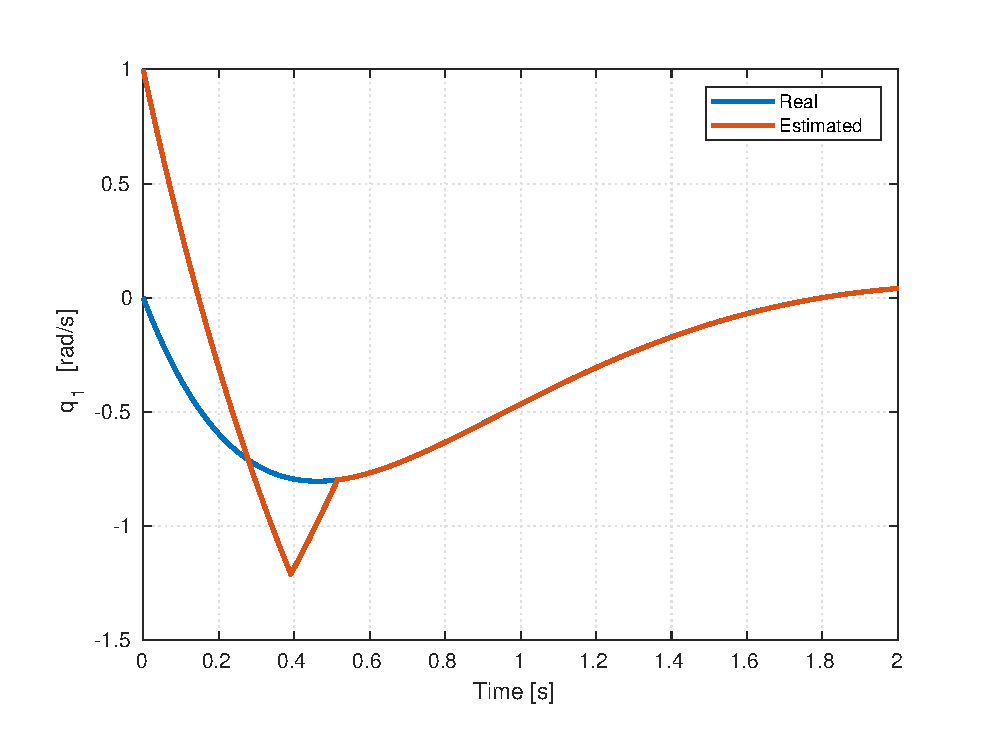
\includegraphics[width=0.5\textwidth]{Figures/est_q1.eps}  
\end{frame}

\begin{frame}\frametitle{Next Steps}
\begin{itemize}
\item Estimate the model parameters (still need to determine if doing it by SM techniques or some other approach)
\item Consider the sampling time of $q$
\item Consider dry friction in the model.
\item Export to ROS Nodes
\end{itemize}  
\end{frame}
\end{document} 
